% Options for packages loaded elsewhere
\PassOptionsToPackage{unicode}{hyperref}
\PassOptionsToPackage{hyphens}{url}
\PassOptionsToPackage{dvipsnames,svgnames*,x11names*}{xcolor}
%
\documentclass[
]{article}
\usepackage{lmodern}
\usepackage{amssymb,amsmath}
\usepackage{ifxetex,ifluatex}
\ifnum 0\ifxetex 1\fi\ifluatex 1\fi=0 % if pdftex
  \usepackage[T1]{fontenc}
  \usepackage[utf8]{inputenc}
  \usepackage{textcomp} % provide euro and other symbols
\else % if luatex or xetex
  \usepackage{unicode-math}
  \defaultfontfeatures{Scale=MatchLowercase}
  \defaultfontfeatures[\rmfamily]{Ligatures=TeX,Scale=1}
\fi
% Use upquote if available, for straight quotes in verbatim environments
\IfFileExists{upquote.sty}{\usepackage{upquote}}{}
\IfFileExists{microtype.sty}{% use microtype if available
  \usepackage[]{microtype}
  \UseMicrotypeSet[protrusion]{basicmath} % disable protrusion for tt fonts
}{}
\makeatletter
\@ifundefined{KOMAClassName}{% if non-KOMA class
  \IfFileExists{parskip.sty}{%
    \usepackage{parskip}
  }{% else
    \setlength{\parindent}{0pt}
    \setlength{\parskip}{6pt plus 2pt minus 1pt}}
}{% if KOMA class
  \KOMAoptions{parskip=half}}
\makeatother
\usepackage{xcolor}
\IfFileExists{xurl.sty}{\usepackage{xurl}}{} % add URL line breaks if available
\IfFileExists{bookmark.sty}{\usepackage{bookmark}}{\usepackage{hyperref}}
\hypersetup{
  pdftitle={ST 790 Assignment 1},
  pdfauthor={David Elsheimer and Jimmy Hickey},
  colorlinks=true,
  linkcolor=Maroon,
  filecolor=Maroon,
  citecolor=Blue,
  urlcolor=blue,
  pdfcreator={LaTeX via pandoc}}
\urlstyle{same} % disable monospaced font for URLs
\usepackage[margin=1in]{geometry}
\usepackage{color}
\usepackage{fancyvrb}
\newcommand{\VerbBar}{|}
\newcommand{\VERB}{\Verb[commandchars=\\\{\}]}
\DefineVerbatimEnvironment{Highlighting}{Verbatim}{commandchars=\\\{\}}
% Add ',fontsize=\small' for more characters per line
\usepackage{framed}
\definecolor{shadecolor}{RGB}{248,248,248}
\newenvironment{Shaded}{\begin{snugshade}}{\end{snugshade}}
\newcommand{\AlertTok}[1]{\textcolor[rgb]{0.94,0.16,0.16}{#1}}
\newcommand{\AnnotationTok}[1]{\textcolor[rgb]{0.56,0.35,0.01}{\textbf{\textit{#1}}}}
\newcommand{\AttributeTok}[1]{\textcolor[rgb]{0.77,0.63,0.00}{#1}}
\newcommand{\BaseNTok}[1]{\textcolor[rgb]{0.00,0.00,0.81}{#1}}
\newcommand{\BuiltInTok}[1]{#1}
\newcommand{\CharTok}[1]{\textcolor[rgb]{0.31,0.60,0.02}{#1}}
\newcommand{\CommentTok}[1]{\textcolor[rgb]{0.56,0.35,0.01}{\textit{#1}}}
\newcommand{\CommentVarTok}[1]{\textcolor[rgb]{0.56,0.35,0.01}{\textbf{\textit{#1}}}}
\newcommand{\ConstantTok}[1]{\textcolor[rgb]{0.00,0.00,0.00}{#1}}
\newcommand{\ControlFlowTok}[1]{\textcolor[rgb]{0.13,0.29,0.53}{\textbf{#1}}}
\newcommand{\DataTypeTok}[1]{\textcolor[rgb]{0.13,0.29,0.53}{#1}}
\newcommand{\DecValTok}[1]{\textcolor[rgb]{0.00,0.00,0.81}{#1}}
\newcommand{\DocumentationTok}[1]{\textcolor[rgb]{0.56,0.35,0.01}{\textbf{\textit{#1}}}}
\newcommand{\ErrorTok}[1]{\textcolor[rgb]{0.64,0.00,0.00}{\textbf{#1}}}
\newcommand{\ExtensionTok}[1]{#1}
\newcommand{\FloatTok}[1]{\textcolor[rgb]{0.00,0.00,0.81}{#1}}
\newcommand{\FunctionTok}[1]{\textcolor[rgb]{0.00,0.00,0.00}{#1}}
\newcommand{\ImportTok}[1]{#1}
\newcommand{\InformationTok}[1]{\textcolor[rgb]{0.56,0.35,0.01}{\textbf{\textit{#1}}}}
\newcommand{\KeywordTok}[1]{\textcolor[rgb]{0.13,0.29,0.53}{\textbf{#1}}}
\newcommand{\NormalTok}[1]{#1}
\newcommand{\OperatorTok}[1]{\textcolor[rgb]{0.81,0.36,0.00}{\textbf{#1}}}
\newcommand{\OtherTok}[1]{\textcolor[rgb]{0.56,0.35,0.01}{#1}}
\newcommand{\PreprocessorTok}[1]{\textcolor[rgb]{0.56,0.35,0.01}{\textit{#1}}}
\newcommand{\RegionMarkerTok}[1]{#1}
\newcommand{\SpecialCharTok}[1]{\textcolor[rgb]{0.00,0.00,0.00}{#1}}
\newcommand{\SpecialStringTok}[1]{\textcolor[rgb]{0.31,0.60,0.02}{#1}}
\newcommand{\StringTok}[1]{\textcolor[rgb]{0.31,0.60,0.02}{#1}}
\newcommand{\VariableTok}[1]{\textcolor[rgb]{0.00,0.00,0.00}{#1}}
\newcommand{\VerbatimStringTok}[1]{\textcolor[rgb]{0.31,0.60,0.02}{#1}}
\newcommand{\WarningTok}[1]{\textcolor[rgb]{0.56,0.35,0.01}{\textbf{\textit{#1}}}}
\usepackage{graphicx,grffile}
\makeatletter
\def\maxwidth{\ifdim\Gin@nat@width>\linewidth\linewidth\else\Gin@nat@width\fi}
\def\maxheight{\ifdim\Gin@nat@height>\textheight\textheight\else\Gin@nat@height\fi}
\makeatother
% Scale images if necessary, so that they will not overflow the page
% margins by default, and it is still possible to overwrite the defaults
% using explicit options in \includegraphics[width, height, ...]{}
\setkeys{Gin}{width=\maxwidth,height=\maxheight,keepaspectratio}
% Set default figure placement to htbp
\makeatletter
\def\fps@figure{htbp}
\makeatother
\setlength{\emergencystretch}{3em} % prevent overfull lines
\providecommand{\tightlist}{%
  \setlength{\itemsep}{0pt}\setlength{\parskip}{0pt}}
\setcounter{secnumdepth}{-\maxdimen} % remove section numbering

\title{ST 790 Assignment 1}
\author{David Elsheimer and Jimmy Hickey}
\date{9/1/2020}

\begin{document}
\maketitle

\hypertarget{instruction}{%
\subsection{Instruction}\label{instruction}}

This assignment consists of \(4\) problems. The assignment is due on
\textbf{Tuesday, September 1} at 11:59pm EDT. Please submit your
assignment electronically through the \textbf{Moodle} webpage. The
assignment can be done as a group with at most 3 members per group
(please include the name of the group members on the front page of the
assignment).

\hypertarget{problem-1}{%
\section{Problem 1}\label{problem-1}}

Download the political blogs dataset from
\href{http://www-personal.umich.edu/~mejn/netdata/}{here}. Now find the
say, top ten, most ``central'' or ``important'' vertices via e.g.,
closeness centrality, betweeness centrality, Katz centrality, page-rank
centrality, and hubs/authority centrality. Does the blogs that you
identified similar to that in Table 1 through Table 3 of
\href{http://www.ramb.ethz.ch/CDstore/www2005-ws/workshop/wf10/AdamicGlanceBlogWWW.pdf}{Adamic
and Glance} ?

\hypertarget{different-centrality-metric-rankings-overall-liberal-conservative}{%
\section{Different Centrality Metric Rankings (Overall, Liberal, \&
Conservative)}\label{different-centrality-metric-rankings-overall-liberal-conservative}}

\begin{Shaded}
\begin{Highlighting}[]
\NormalTok{g<-}\KeywordTok{read.graph}\NormalTok{(}\StringTok{"polblogs.gml"}\NormalTok{,}\DataTypeTok{format=}\KeywordTok{c}\NormalTok{(}\StringTok{"gml"}\NormalTok{))}
\KeywordTok{summary}\NormalTok{(g)}
\end{Highlighting}
\end{Shaded}

\begin{verbatim}
## IGRAPH 80c8502 D--- 1490 19090 -- 
## + attr: id (v/n), label (v/c), value (v/n), source (v/c)
\end{verbatim}

\begin{Shaded}
\begin{Highlighting}[]
\NormalTok{labels <-}\StringTok{ }\KeywordTok{V}\NormalTok{(g)}\OperatorTok{$}\NormalTok{label}
\NormalTok{val <-}\StringTok{ }\KeywordTok{V}\NormalTok{(g)}\OperatorTok{$}\NormalTok{value}

\NormalTok{closeness <-}\StringTok{ }\KeywordTok{closeness}\NormalTok{(g)}
\NormalTok{betweenness <-}\StringTok{ }\KeywordTok{betweenness}\NormalTok{(g)}
\NormalTok{pg <-}\StringTok{ }\KeywordTok{page_rank}\NormalTok{(g)}\OperatorTok{$}\NormalTok{vector}
\NormalTok{katz <-}\StringTok{ }\KeywordTok{alpha_centrality}\NormalTok{(g, }\DataTypeTok{alpha =} \FloatTok{0.05}\NormalTok{)}
\NormalTok{hub <-}\StringTok{ }\KeywordTok{hub_score}\NormalTok{(g)}\OperatorTok{$}\NormalTok{vector}
\NormalTok{auth <-}\StringTok{ }\KeywordTok{authority_score}\NormalTok{(g)}\OperatorTok{$}\NormalTok{vector}

\NormalTok{nodeinfo <-}\StringTok{ }\KeywordTok{as.data.frame}\NormalTok{(labels)}
\NormalTok{nodeinfo <-}\StringTok{ }\KeywordTok{mutate}\NormalTok{(nodeinfo, }\DataTypeTok{val =}\NormalTok{ val, }\DataTypeTok{close=}\NormalTok{closeness, }\DataTypeTok{between=}\NormalTok{betweenness, }\DataTypeTok{pg =}\NormalTok{ pg, }
                   \DataTypeTok{katz =}\NormalTok{ katz, }\DataTypeTok{hub =}\NormalTok{ hub, }\DataTypeTok{auth =}\NormalTok{ auth)}

\NormalTok{pgrank    <-}\StringTok{ }\NormalTok{nodeinfo }\OperatorTok\StringTok{ }\KeywordTok{arrange}\NormalTok{(}\KeywordTok{desc}\NormalTok{(close)) }\OperatorTok\StringTok{  }\KeywordTok{select}\NormalTok{(labels) }\OperatorTok\KeywordTok{head}\NormalTok{(}\DataTypeTok{n=}\DecValTok{10}\NormalTok{) }

\NormalTok{pgranklib <-}\StringTok{ }\NormalTok{nodeinfo }\OperatorTok\StringTok{ }\KeywordTok{filter}\NormalTok{(val }\OperatorTok{==}\StringTok{ }\DecValTok{0}\NormalTok{) }\OperatorTok\StringTok{ }
\StringTok{  }\KeywordTok{arrange}\NormalTok{(}\KeywordTok{desc}\NormalTok{(pg)) }\OperatorTok\StringTok{  }\KeywordTok{select}\NormalTok{(labels) }\OperatorTok\KeywordTok{head}\NormalTok{(}\DataTypeTok{n=}\DecValTok{10}\NormalTok{) }

\NormalTok{pgrankcon <-}\StringTok{ }\NormalTok{nodeinfo }\OperatorTok\StringTok{ }\KeywordTok{filter}\NormalTok{(val }\OperatorTok{==}\StringTok{ }\DecValTok{1}\NormalTok{) }\OperatorTok\StringTok{ }
\StringTok{  }\KeywordTok{arrange}\NormalTok{(}\KeywordTok{desc}\NormalTok{(pg)) }\OperatorTok\StringTok{  }\KeywordTok{select}\NormalTok{(labels) }\OperatorTok\KeywordTok{head}\NormalTok{(}\DataTypeTok{n=}\DecValTok{10}\NormalTok{) }


\NormalTok{closerank    <-}\StringTok{ }\NormalTok{nodeinfo }\OperatorTok\StringTok{ }\KeywordTok{arrange}\NormalTok{(}\KeywordTok{desc}\NormalTok{(close)) }\OperatorTok\StringTok{  }\KeywordTok{select}\NormalTok{(labels) }\OperatorTok\KeywordTok{head}\NormalTok{(}\DataTypeTok{n=}\DecValTok{10}\NormalTok{) }

\NormalTok{closeranklib <-}\StringTok{ }\NormalTok{nodeinfo }\OperatorTok\StringTok{ }\KeywordTok{filter}\NormalTok{(val }\OperatorTok{==}\StringTok{ }\DecValTok{0}\NormalTok{) }\OperatorTok\StringTok{ }
\StringTok{  }\KeywordTok{arrange}\NormalTok{(}\KeywordTok{desc}\NormalTok{(close)) }\OperatorTok\StringTok{  }\KeywordTok{select}\NormalTok{(labels) }\OperatorTok\KeywordTok{head}\NormalTok{(}\DataTypeTok{n=}\DecValTok{10}\NormalTok{) }

\NormalTok{closerankcon <-}\StringTok{ }\NormalTok{nodeinfo }\OperatorTok\StringTok{ }\KeywordTok{filter}\NormalTok{(val }\OperatorTok{==}\StringTok{ }\DecValTok{1}\NormalTok{) }\OperatorTok\StringTok{ }
\StringTok{  }\KeywordTok{arrange}\NormalTok{(}\KeywordTok{desc}\NormalTok{(close)) }\OperatorTok\StringTok{  }\KeywordTok{select}\NormalTok{(labels) }\OperatorTok\KeywordTok{head}\NormalTok{(}\DataTypeTok{n=}\DecValTok{10}\NormalTok{) }


\NormalTok{betweenrank    <-}\StringTok{ }\NormalTok{nodeinfo }\OperatorTok\StringTok{ }\KeywordTok{arrange}\NormalTok{(}\KeywordTok{desc}\NormalTok{(between)) }\OperatorTok\StringTok{  }\KeywordTok{select}\NormalTok{(labels) }\OperatorTok\KeywordTok{head}\NormalTok{(}\DataTypeTok{n=}\DecValTok{10}\NormalTok{) }

\NormalTok{betweenranklib <-}\StringTok{ }\NormalTok{nodeinfo }\OperatorTok\StringTok{ }\KeywordTok{filter}\NormalTok{(val }\OperatorTok{==}\StringTok{ }\DecValTok{0}\NormalTok{) }\OperatorTok
\StringTok{  }\KeywordTok{arrange}\NormalTok{(}\KeywordTok{desc}\NormalTok{(between)) }\OperatorTok\StringTok{  }\KeywordTok{select}\NormalTok{(labels) }\OperatorTok\KeywordTok{head}\NormalTok{(}\DataTypeTok{n=}\DecValTok{10}\NormalTok{) }

\NormalTok{betweenrankcon <-}\StringTok{ }\NormalTok{nodeinfo }\OperatorTok\StringTok{ }\KeywordTok{filter}\NormalTok{(val }\OperatorTok{==}\StringTok{ }\DecValTok{1}\NormalTok{) }\OperatorTok\StringTok{ }
\StringTok{  }\KeywordTok{arrange}\NormalTok{(}\KeywordTok{desc}\NormalTok{(between)) }\OperatorTok\StringTok{  }\KeywordTok{select}\NormalTok{(labels) }\OperatorTok\KeywordTok{head}\NormalTok{(}\DataTypeTok{n=}\DecValTok{10}\NormalTok{)}

\NormalTok{katzrank    <-}\StringTok{ }\NormalTok{nodeinfo }\OperatorTok\StringTok{ }\KeywordTok{arrange}\NormalTok{(}\KeywordTok{desc}\NormalTok{(katz)) }\OperatorTok\StringTok{  }\KeywordTok{select}\NormalTok{(labels) }\OperatorTok\KeywordTok{head}\NormalTok{(}\DataTypeTok{n=}\DecValTok{10}\NormalTok{) }

\NormalTok{katzranklib <-}\StringTok{ }\NormalTok{nodeinfo }\OperatorTok\StringTok{ }\KeywordTok{filter}\NormalTok{(val }\OperatorTok{==}\StringTok{ }\DecValTok{0}\NormalTok{) }\OperatorTok\StringTok{ }
\StringTok{  }\KeywordTok{arrange}\NormalTok{(}\KeywordTok{desc}\NormalTok{(katz)) }\OperatorTok\StringTok{  }\KeywordTok{select}\NormalTok{(labels) }\OperatorTok\KeywordTok{head}\NormalTok{(}\DataTypeTok{n=}\DecValTok{10}\NormalTok{) }

\NormalTok{katzrankcon <-}\StringTok{ }\NormalTok{nodeinfo }\OperatorTok\StringTok{ }\KeywordTok{filter}\NormalTok{(val }\OperatorTok{==}\StringTok{ }\DecValTok{1}\NormalTok{) }\OperatorTok\StringTok{ }
\StringTok{  }\KeywordTok{arrange}\NormalTok{(}\KeywordTok{desc}\NormalTok{(katz)) }\OperatorTok\StringTok{  }\KeywordTok{select}\NormalTok{(labels) }\OperatorTok\KeywordTok{head}\NormalTok{(}\DataTypeTok{n=}\DecValTok{10}\NormalTok{)}

\NormalTok{hubrank    <-}\StringTok{ }\NormalTok{nodeinfo }\OperatorTok\StringTok{ }\KeywordTok{arrange}\NormalTok{(}\KeywordTok{desc}\NormalTok{(hub)) }\OperatorTok\StringTok{  }\KeywordTok{select}\NormalTok{(labels) }\OperatorTok\KeywordTok{head}\NormalTok{(}\DataTypeTok{n=}\DecValTok{10}\NormalTok{) }

\NormalTok{hubranklib <-}\StringTok{ }\NormalTok{nodeinfo }\OperatorTok\StringTok{ }\KeywordTok{filter}\NormalTok{(val }\OperatorTok{==}\StringTok{ }\DecValTok{0}\NormalTok{) }\OperatorTok\StringTok{ }
\StringTok{  }\KeywordTok{arrange}\NormalTok{(}\KeywordTok{desc}\NormalTok{(hub)) }\OperatorTok\StringTok{  }\KeywordTok{select}\NormalTok{(labels) }\OperatorTok\KeywordTok{head}\NormalTok{(}\DataTypeTok{n=}\DecValTok{10}\NormalTok{) }

\NormalTok{hubrankcon <-}\StringTok{ }\NormalTok{nodeinfo }\OperatorTok\StringTok{ }\KeywordTok{filter}\NormalTok{(val }\OperatorTok{==}\StringTok{ }\DecValTok{1}\NormalTok{) }\OperatorTok
\StringTok{  }\KeywordTok{arrange}\NormalTok{(}\KeywordTok{desc}\NormalTok{(hub)) }\OperatorTok\StringTok{  }\KeywordTok{select}\NormalTok{(labels) }\OperatorTok\KeywordTok{head}\NormalTok{(}\DataTypeTok{n=}\DecValTok{10}\NormalTok{)}



\NormalTok{authrank    <-}\StringTok{ }\NormalTok{nodeinfo }\OperatorTok\StringTok{ }\KeywordTok{arrange}\NormalTok{(}\KeywordTok{desc}\NormalTok{(auth)) }\OperatorTok\StringTok{  }\KeywordTok{select}\NormalTok{(labels) }\OperatorTok\KeywordTok{head}\NormalTok{(}\DataTypeTok{n=}\DecValTok{10}\NormalTok{) }

\NormalTok{authranklib <-}\StringTok{ }\NormalTok{nodeinfo }\OperatorTok\StringTok{ }\KeywordTok{filter}\NormalTok{(val }\OperatorTok{==}\StringTok{ }\DecValTok{0}\NormalTok{) }\OperatorTok\StringTok{ }
\StringTok{  }\KeywordTok{arrange}\NormalTok{(}\KeywordTok{desc}\NormalTok{(auth)) }\OperatorTok\StringTok{  }\KeywordTok{select}\NormalTok{(labels) }\OperatorTok\KeywordTok{head}\NormalTok{(}\DataTypeTok{n=}\DecValTok{10}\NormalTok{) }

\NormalTok{authrankcon <-}\StringTok{ }\NormalTok{nodeinfo }\OperatorTok\StringTok{ }\KeywordTok{filter}\NormalTok{(val }\OperatorTok{==}\StringTok{ }\DecValTok{1}\NormalTok{) }\OperatorTok
\StringTok{  }\KeywordTok{arrange}\NormalTok{(}\KeywordTok{desc}\NormalTok{(auth)) }\OperatorTok\StringTok{  }\KeywordTok{select}\NormalTok{(labels) }\OperatorTok\KeywordTok{head}\NormalTok{(}\DataTypeTok{n=}\DecValTok{10}\NormalTok{)}

\NormalTok{rankings1 <-}\StringTok{ }\KeywordTok{as.data.frame}\NormalTok{(}\KeywordTok{cbind}\NormalTok{(pgrank, closerank, betweenrank))}

\NormalTok{rankings2 <-}\StringTok{ }\KeywordTok{as.data.frame}\NormalTok{(}\KeywordTok{cbind}\NormalTok{(katzrank, hubrank, authrank))}
\KeywordTok{colnames}\NormalTok{(rankings1) <-}\StringTok{ }\KeywordTok{c}\NormalTok{(}\StringTok{"Page rank"}\NormalTok{, }\StringTok{"Closeness"}\NormalTok{, }\StringTok{"Betweeness"}\NormalTok{)}
\KeywordTok{colnames}\NormalTok{(rankings2) <-}\StringTok{ }\KeywordTok{c}\NormalTok{(}\StringTok{"Katz"}\NormalTok{, }\StringTok{"Hub"}\NormalTok{, }\StringTok{"Authority"}\NormalTok{)}

\NormalTok{librankings1 <-}\StringTok{ }\KeywordTok{as.data.frame}\NormalTok{(}\KeywordTok{cbind}\NormalTok{(pgranklib, closeranklib, betweenranklib))}

\NormalTok{librankings2 <-}\StringTok{ }\KeywordTok{as.data.frame}\NormalTok{(}\KeywordTok{cbind}\NormalTok{(katzranklib, hubranklib, authranklib))}
\KeywordTok{colnames}\NormalTok{(librankings1) <-}\StringTok{ }\KeywordTok{c}\NormalTok{(}\StringTok{"Page rank"}\NormalTok{, }\StringTok{"Closeness"}\NormalTok{, }\StringTok{"Betweeness"}\NormalTok{)}
\KeywordTok{colnames}\NormalTok{(librankings2) <-}\StringTok{ }\KeywordTok{c}\NormalTok{(}\StringTok{"Katz"}\NormalTok{, }\StringTok{"Hub"}\NormalTok{, }\StringTok{"Authority"}\NormalTok{)}

\NormalTok{conrankings1 <-}\StringTok{ }\KeywordTok{as.data.frame}\NormalTok{(}\KeywordTok{cbind}\NormalTok{(pgrankcon, closerankcon, betweenrankcon))}

\NormalTok{conrankings2 <-}\StringTok{ }\KeywordTok{as.data.frame}\NormalTok{(}\KeywordTok{cbind}\NormalTok{(katzrankcon, hubrankcon, authrankcon))}
\KeywordTok{colnames}\NormalTok{(conrankings1) <-}\StringTok{ }\KeywordTok{c}\NormalTok{(}\StringTok{"Page rank"}\NormalTok{, }\StringTok{"Closeness"}\NormalTok{, }\StringTok{"Betweeness"}\NormalTok{)}
\KeywordTok{colnames}\NormalTok{(conrankings2) <-}\StringTok{ }\KeywordTok{c}\NormalTok{(}\StringTok{"Katz"}\NormalTok{, }\StringTok{"Hub"}\NormalTok{, }\StringTok{"Authority"}\NormalTok{)}
\end{Highlighting}
\end{Shaded}

\hypertarget{overall}{%
\subsection{Overall}\label{overall}}

\begin{table}[ht]
\centering
\begin{tabular}{rlll}
  \hline
 & Page rank & Closeness & Betweeness \\ 
  \hline
1 & itlookslikethis.blogeasy.com & itlookslikethis.blogeasy.com & blogsforbush.com \\ 
  2 & bushmisunderestimated.blogspot.com & bushmisunderestimated.blogspot.com & atrios.blogspot.com \\ 
  3 & etherealgirl.blogspot.com & etherealgirl.blogspot.com & instapundit.com \\ 
  4 & michaelphillips.blogspot.com & michaelphillips.blogspot.com & dailykos.com \\ 
  5 & lennonreport.blogspot.com & lennonreport.blogspot.com & newleftblogs.blogspot.com \\ 
  6 & isdl.blogspot.com & isdl.blogspot.com & madkane.com/notable.html \\ 
  7 & isdl.weblogs.us & isdl.weblogs.us & wizbangblog.com \\ 
  8 & janm.blogspot.com & janm.blogspot.com & lashawnbarber.com \\ 
  9 & nerofiddled.blogspot.com & nerofiddled.blogspot.com & hughhewitt.com \\ 
  10 & saveoursenate.blogspot.com & saveoursenate.blogspot.com & washingtonmonthly.com \\ 
   \hline
\end{tabular}
\end{table}
\begin{table}[ht]
\centering
\begin{tabular}{rlll}
  \hline
 & Katz & Hub & Authority \\ 
  \hline
1 & rooksrant.com & politicalstrategy.org & dailykos.com \\ 
  2 & blogsagainsthillary.com & madkane.com/notable.html & talkingpointsmemo.com \\ 
  3 & burntorangereport.com & liberaloasis.com & atrios.blogspot.com \\ 
  4 & collegedems.com/blog & stagefour.typepad.com/commonprejudice & washingtonmonthly.com \\ 
  5 & gregpalast.com & bodyandsoul.typepad.com & talkleft.com \\ 
  6 & bopnews.com & corrente.blogspot.com & instapundit.com \\ 
  7 & rudepundit.blogspot.com & atrios.blogspot.com/  & juancole.com \\ 
  8 & iddybud.blogspot.com & tbogg.blogspot.com & yglesias.typepad.com/matthew \\ 
  9 & shakespearessister.blogspot.com & newleftblogs.blogspot.com & pandagon.net \\ 
  10 & home.earthlink.net/\~{}fsrhine & atrios.blogspot.com & digbysblog.blogspot.com \\ 
   \hline
\end{tabular}
\end{table}
\newpage

\hypertarget{liberal}{%
\subsection{Liberal}\label{liberal}}

\begin{table}[ht]
\centering
\begin{tabular}{rlll}
  \hline
 & Page rank & Closeness & Betweeness \\ 
  \hline
1 & dailykos.com & itlookslikethis.blogeasy.com & atrios.blogspot.com \\ 
  2 & atrios.blogspot.com & bushmisunderestimated.blogspot.com & dailykos.com \\ 
  3 & talkingpointsmemo.com & etherealgirl.blogspot.com & newleftblogs.blogspot.com \\ 
  4 & washingtonmonthly.com & michaelphillips.blogspot.com & madkane.com/notable.html \\ 
  5 & juancole.com & lennonreport.blogspot.com & washingtonmonthly.com \\ 
  6 & prospect.org/weblog & janm.blogspot.com & liberaloasis.com \\ 
  7 & digbysblog.blogspot.com & nerofiddled.blogspot.com & digbysblog.blogspot.com \\ 
  8 & talkleft.com & saveoursenate.blogspot.com & robschumacher.blogspot.com \\ 
  9 & yglesias.typepad.com/matthew & dashnier.blogspot.com & nomoremister.blogspot.com \\ 
  10 & jameswolcott.com & politicalmonitor.us/blog & xnerg.blogspot.com \\ 
   \hline
\end{tabular}
\end{table}

\begin{table}[ht]
\centering
\begin{tabular}{rlll}
  \hline
 & Katz & Hub & Authority \\ 
  \hline
1 & rooksrant.com & politicalstrategy.org & dailykos.com \\ 
  2 & burntorangereport.com & madkane.com/notable.html & talkingpointsmemo.com \\ 
  3 & collegedems.com/blog & liberaloasis.com & atrios.blogspot.com \\ 
  4 & gregpalast.com & stagefour.typepad.com/commonprejudice & washingtonmonthly.com \\ 
  5 & bopnews.com & bodyandsoul.typepad.com & talkleft.com \\ 
  6 & rudepundit.blogspot.com & corrente.blogspot.com & juancole.com \\ 
  7 & iddybud.blogspot.com & atrios.blogspot.com/  & yglesias.typepad.com/matthew \\ 
  8 & shakespearessister.blogspot.com & tbogg.blogspot.com & pandagon.net \\ 
  9 & home.earthlink.net/\~{}fsrhine & newleftblogs.blogspot.com & digbysblog.blogspot.com \\ 
  10 & mahablog.com & atrios.blogspot.com & prospect.org/weblog \\ 
   \hline
\end{tabular}
\end{table}
\newpage

\hypertarget{conservative}{%
\subsection{Conservative}\label{conservative}}

\begin{table}[ht]
\centering
\begin{tabular}{rlll}
  \hline
 & Page rank & Closeness & Betweeness \\ 
  \hline
1 & instapundit.com & isdl.blogspot.com & blogsforbush.com \\ 
  2 & blogsforbush.com & isdl.weblogs.us & instapundit.com \\ 
  3 & michellemalkin.com & streetlog.typepad.com & wizbangblog.com \\ 
  4 & drudgereport.com & rednyc.blogspot.com & lashawnbarber.com \\ 
  5 & powerlineblog.com & r2korn.blogdrive.com & hughhewitt.com \\ 
  6 & andrewsullivan.com & thelastword.blogdrive.com & gevkaffeegal.typepad.com/the\_alliance \\ 
  7 & littlegreenfootballs.com/weblog & calirep.blogspot.com & michellemalkin.com \\ 
  8 & vodkapundit.com & smashingzero.blogspot.com & truthlaidbear.com \\ 
  9 & rightwingnews.com & lonewacko.com & littlegreenfootballs.com/weblog \\ 
  10 & volokh.com & nicoladellarciprete.blogs.com & evangelicaloutpost.com \\ 
   \hline
\end{tabular}
\end{table}
\begin{table}[ht]
\centering
\begin{tabular}{rlll}
  \hline
 & Katz & Hub & Authority \\ 
  \hline
1 & blogsagainsthillary.com & instapundit.com & instapundit.com \\ 
  2 & etalkinghead.com & dalythoughts.com & powerlineblog.com \\ 
  3 & nickiegoomba.blogspot.com & acertainslantoflight.blogspot.com & andrewsullivan.com \\ 
  4 & swiftreport.blogs.com & incite1.blogspot.com & truthlaidbear.com \\ 
  5 & stmonk.blogspot.com & thomasgalvin.blogspot.com & michellemalkin.com \\ 
  6 & poeticvalues.blogspot.com & truthprobe.blogspot.com & drudgereport.com \\ 
  7 & thejessefactor.blogspot.com & blogsofwar.com & nationalreview.com/thecorner \\ 
  8 & conservativepunk.com & scha-den-freu-de.blogspot.com & littlegreenfootballs.com/weblog \\ 
  9 & zebrax.blogs.com & vodkapundit.com & hughhewitt.com \\ 
  10 & dizzy-girl.net/index.php & cayankee.blogs.com & volokh.com \\ 
   \hline
\end{tabular}
\end{table}

Using the page rank metric, the top 10 blocks for liberal and
conservative are similar for to those in tables 1 and 2. The top 10 vary
based on the metric chosen, but several other top 10 rankings are
similar as well. For example, the authority and betweeness centrality
metrics are fair similar for conservative blogs as well as liberal
blogs. For the overall rankings (table 3 in the paper), the metrics used
to rank blogs are unclear. There does appear to be some consensus
between the different centrality metrics, however.

\hypertarget{problem-2}{%
\section{Problem 2}\label{problem-2}}

Skim through this \href{https://arxiv.org/pdf/0706.1062.pdf}{article} by
Clauset, Shalizi, and Newman. Now download the yeast metabolic network
dataset from
\href{http://tuvalu.santafe.edu/~aaronc/powerlaws/data.htm}{here}. Fit a
power-law to the degree distribution for this dataset. Do you think the
degree distribution for this network follows a power-law ?

\begin{Shaded}
\begin{Highlighting}[]
\KeywordTok{library}\NormalTok{(igraph)}
\NormalTok{g2 <-}\StringTok{ }\KeywordTok{read_graph}\NormalTok{(}\StringTok{"nodes.txt"}\NormalTok{)}
\NormalTok{cg <-}\StringTok{ }\KeywordTok{components}\NormalTok{(g2)}
\NormalTok{lcc <-}\StringTok{ }\KeywordTok{decompose}\NormalTok{(g2, }\DataTypeTok{min.vertices =} \KeywordTok{max}\NormalTok{(cg}\OperatorTok{$}\NormalTok{csize))[[}\DecValTok{1}\NormalTok{]];}

\NormalTok{deg_dist <-}\StringTok{ }\KeywordTok{degree_distribution}\NormalTok{(lcc, }\DataTypeTok{cumulative =} \OtherTok{TRUE}\NormalTok{)}
\NormalTok{mod <-}\StringTok{ }\KeywordTok{lm}\NormalTok{(}\KeywordTok{log}\NormalTok{(deg_dist,}\DecValTok{10}\NormalTok{) }\OperatorTok{~}\StringTok{ }\KeywordTok{log}\NormalTok{(}\DecValTok{1}\OperatorTok{:}\KeywordTok{length}\NormalTok{(deg_dist),}\DecValTok{10}\NormalTok{))}
\NormalTok{mod}\OperatorTok{$}\NormalTok{coefficients }\CommentTok{##``Estimate'' of exponent in power-law}
\end{Highlighting}
\end{Shaded}

\begin{verbatim}
##                 (Intercept) log(1:length(deg_dist), 10) 
##                   0.8195035                  -2.3120220
\end{verbatim}

\begin{Shaded}
\begin{Highlighting}[]
\KeywordTok{plot}\NormalTok{(}\KeywordTok{log}\NormalTok{(}\DecValTok{1}\OperatorTok{:}\KeywordTok{length}\NormalTok{(deg_dist),}\DecValTok{10}\NormalTok{),}\KeywordTok{log}\NormalTok{(deg_dist,}\DecValTok{10}\NormalTok{),}
\DataTypeTok{xlab =} \StringTok{"degree (log-scale)"}\NormalTok{, }\DataTypeTok{ylab =} \StringTok{"cumulative frequency (log-scale)"}\NormalTok{,}\KeywordTok{abline}\NormalTok{(mod))}
\end{Highlighting}
\end{Shaded}

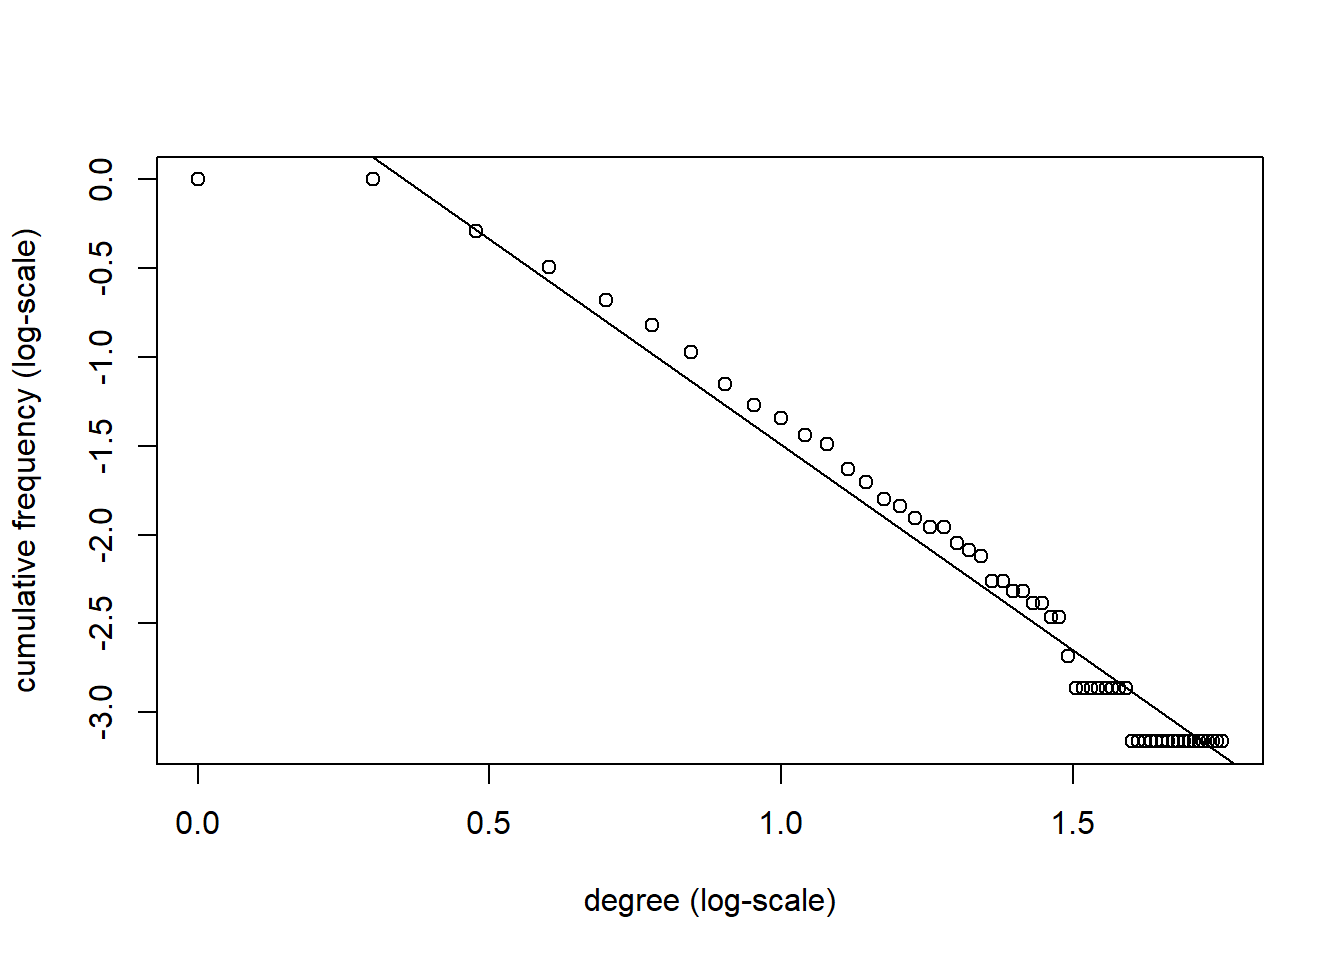
\includegraphics{hw1_files/figure-latex/unnamed-chunk-3-1.pdf} Based on
the above comparison of the data to the fitted power law, it appears
that the degree distribution does indeed follow a power law.

\hypertarget{problem-3}{%
\section{Problem 3}\label{problem-3}}

Let \(X_1, X_2, \dots, X_n\) be i.i.d random variables. The sample
variance of the \(X_i\) can be written as a \(U\)-statistics, i.e.,
\[s^2 = \frac{2}{n(n-1)} \sum_{i < j} \frac{1}{2} (X_i - X_j)^2.\]
Suppose now the \(X_i\) are i.i.d Bernoulli random variables with
probability of success \(p \in (0,1)\). Derive a non-degenerate limiting
distribution for \(s^2\). What happens to this limiting distribution
when \(p = 1/2\) ?

\hypertarget{problem-4}{%
\section{Problem 4}\label{problem-4}}

We now consider the problem of goodness-of-fit test for Erdos-Renyi
graphs. More specifically, let \(\mathcal{G} = \mathcal{G}(n,m,p, q)\)
be a random graph model defined as follows. A graph \(G\) is an instance
of \(\mathcal{G}\) if \(G\) is an undirected graph on \(n\) vertices
with adjacency matrix \(\mathbf{A} = (a_{ij})\) of the form
\begin{gather*}
a_{ij} \sim \mathrm{Bernoulli}(q), \quad \text{if $i \in \mathcal{S}$ and $j \in \mathcal{S}$} \\
a_{ij} \sim \mathrm{Bernoulli}(p), \quad \text{otherwise}.
\end{gather*} Here \(\mathcal{S} \subset \{1,2,\dots,n\}\) is a subset
of vertices with \(|\mathcal{S}| = m\) and we have assumed that
\(q > p \in (0,1)\). Note that \(m = 0\) corresponds to the normal
Erdos-Renyi graph and \(m > 0\) corresponds to a random graph model
where there is a subset \(\mathcal{S}\) of \(m\) vertices with larger
communication probability \(q\) among themselves.

Given a graph \(G \sim \mathcal{G}(n,m,p,q)\), we are interested in
testing the null hypothesis
\(\mathbb{H}_0 \colon |\mathcal{S}| = m = 0\) against the alternative
hypothesis that \(\mathbb{H}_A \colon |\mathcal{S}| = m > 0\).

For this problem, we will use two test statistics. The first test
statistic is \(\Delta\), the maximum degree and the second test
statistic is \(\tau\), the number of triangles. More specifically, given
a graph \(G \sim \mathcal{G}(n,m,p,q)\), and suppose we are using
\(\Delta\) as the test statistic. Then we will reject the null
hypothesis if \(\Delta\) exceeds some threshold \(c\).

Perform a simulation study to determine the power of the test procedures
when we use (1) \(\Delta\) as the test statistic and (2) when we use
\(\tau\) as the test statistic. To reduce computation time, set
\(n = 1000\), \(p = 0.4\), and \(q = 0.6\) and let
\(m \in \{10,25,50,100\}\). Report a table for the power of the test
statistics as a function of \(m\).

\textbf{Hint} To generate a graph from the \(\mathcal{G}(n,m,p,q)\) when
\(m > 0\), you can use the following igraph chunk.

\begin{Shaded}
\begin{Highlighting}[]
\KeywordTok{library}\NormalTok{(igraph)}
\NormalTok{p <-}\StringTok{ }\FloatTok{0.4}
\NormalTok{q <-}\StringTok{ }\FloatTok{0.6}
\NormalTok{n <-}\StringTok{ }\DecValTok{1000}
\NormalTok{m <-}\StringTok{ }\DecValTok{10}
\NormalTok{B <-}\StringTok{ }\KeywordTok{matrix}\NormalTok{(}\KeywordTok{c}\NormalTok{(p,p,p,q),}\DataTypeTok{nrow =} \DecValTok{2}\NormalTok{)}
\NormalTok{A <-}\StringTok{ }\KeywordTok{sbm.game}\NormalTok{(}\DataTypeTok{n =}\NormalTok{ n, }\DataTypeTok{pref.matrix =}\NormalTok{ B, }\DataTypeTok{block.sizes =} \KeywordTok{c}\NormalTok{(n}\OperatorTok{-}\NormalTok{m,m))}
\NormalTok{A}
\end{Highlighting}
\end{Shaded}

\begin{verbatim}
## IGRAPH 816854a U--- 1000 200025 -- Stochastic block-model
## + attr: name (g/c), loops (g/l)
## + edges from 816854a:
##  [1]  1-- 2  1-- 3  1-- 5  3-- 6  1-- 7  4-- 7  6-- 7  2-- 8  4-- 8  5-- 8
## [11]  1-- 9  3-- 9  4-- 9  6-- 9  7-- 9  8-- 9  1--10  3--10  5--10  1--11
## [21]  2--11  3--11  4--11  5--11  7--11  8--11 10--11  3--12  5--12  6--12
## [31]  8--12  9--12 10--12 11--12  1--13  2--13  7--13  9--13  1--14  3--14
## [41]  7--14  8--14 12--14 13--14  1--15  2--15  3--15  7--15  8--15 10--15
## [51] 11--15 12--15  2--16  3--16  4--16  7--16  8--16  9--16 12--16 13--16
## [61] 14--16  1--17  4--17  5--17  8--17  9--17 12--17 13--17 14--17  2--18
## [71]  7--18  8--18  9--18 17--18  1--19  5--19  6--19 10--19 11--19 18--19
## + ... omitted several edges
\end{verbatim}

The maximum degree and the number of triangles can be easily determined
via

\begin{Shaded}
\begin{Highlighting}[]
\KeywordTok{max}\NormalTok{(}\KeywordTok{degree}\NormalTok{(A))}
\end{Highlighting}
\end{Shaded}

\begin{verbatim}
## [1] 454
\end{verbatim}

\begin{Shaded}
\begin{Highlighting}[]
\KeywordTok{sum}\NormalTok{(}\KeywordTok{count_triangles}\NormalTok{(A))}\OperatorTok{/}\DecValTok{3}
\end{Highlighting}
\end{Shaded}

\begin{verbatim}
## [1] 10668498
\end{verbatim}

\end{document}
